\documentclass[tikz,border=3pt,convert={density=600,outext=.png}]{standalone}
%\documentclass[tikz,border=3pt]{standalone}

\usepackage[utf8]{inputenc} % utf8 encoding
\usepackage[english]{babel}
\usepackage[T1]{fontenc} % use T1 fonts
\usepackage{amsmath} % nice math symbols

\usepackage{tikz}
\usetikzlibrary{shapes,positioning,calc,arrows,patterns}

\begin{document}
	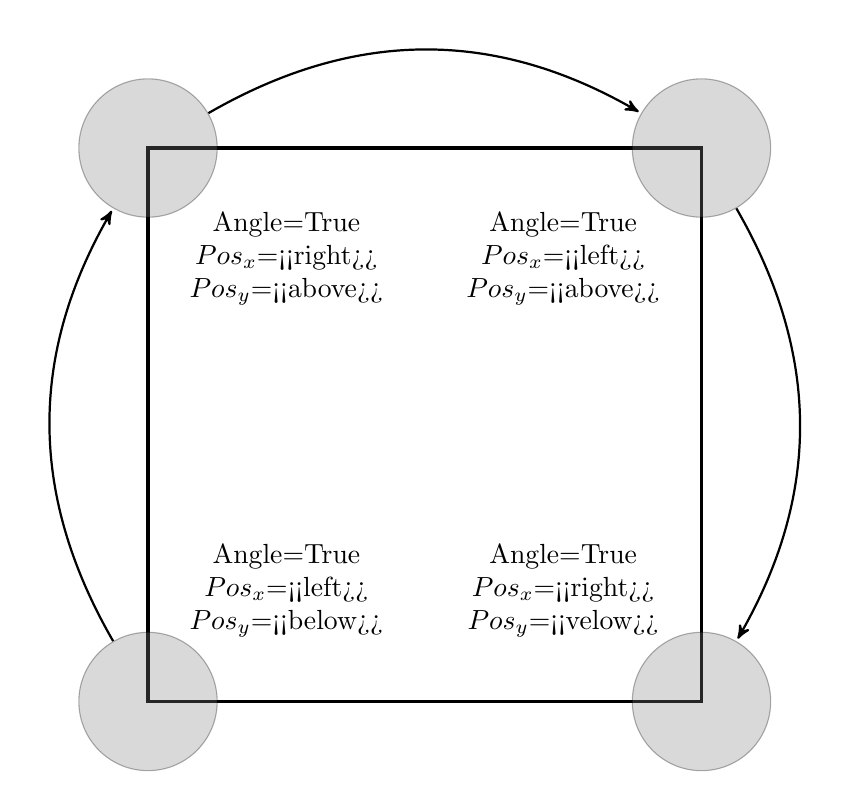
\begin{tikzpicture}[>=triangle 60]
		\node[draw, rectangle, very thick, minimum width=200, minimum height=200] at (0,0) {};
		
		\node[draw, circle, minimum width = 50, fill=gray, opacity=0.3] (a1) at (-100pt,-100pt) {};
		\node[draw, circle, minimum width = 50, fill=gray, opacity=0.3] (a2) at (-100pt,100pt) {};
		\node[draw, circle, minimum width = 50, fill=gray, opacity=0.3] (a3) at (100pt,100pt) {};
		\node[draw, circle, minimum width = 50, fill=gray, opacity=0.3] (a4) at (100pt,-100pt) {};
		
		\node[align=center] at (-50pt, -60pt) {Angle=True\\$Pos_x$=<<left>>\\${Pos_y}$=<<below>>};
		\node[align=center] at (50pt, 60pt) {Angle=True\\$Pos_x$=<<left>>\\${Pos_y}$=<<above>>};
		\node[align=center] at (-50pt, 60pt) {Angle=True\\$Pos_x$=<<right>>\\${Pos_y}$=<<above>>};
		\node[align=center] at (50pt, -60pt) {Angle=True\\$Pos_x$=<<right>>\\${Pos_y}$=<<velow>>};
		
		\draw[->,>=stealth',shorten >=1pt,thick] (a1) edge [bend left] (a2);
		\draw[->,>=stealth',shorten >=1pt,thick] (a2) edge [bend left] (a3);
		\draw[->,>=stealth',shorten >=1pt,thick] (a3) edge [bend left] (a4);

	\end{tikzpicture}
\end{document}
	